\documentclass[class=report, crop=false, 12pt,a4paper]{standalone}
\usepackage{enumitem}
\usepackage{multicol}
\usepackage{graphicx}
\usepackage{float}
\usepackage{amsmath}
\usepackage{amssymb}
\usepackage{mathtools}
\usepackage{siunitx}
\usepackage{commath}
\usepackage{array}
\usepackage{natbib}
\usepackage{tikz}
\usepackage[a4paper,width=150mm,top=25mm,bottom=25mm]{geometry}
\usetikzlibrary{positioning, fit, calc}   
\tikzset{block/.style={draw, thick, text width=3cm ,minimum height=1.3cm, align=center},   
line/.style={-latex}     
}  
\setlength{\parindent}{0pt}
\begin{document}
\section{Boundary Layer Theory}
x-direction:
\begin{align}
  u \frac{\partial u}{\partial x} + v \frac{\partial u}{\partial y} = - \frac{1}{\rho} \frac{\partial p}{\partial x} + \nu \frac{\partial^2 u}{\partial y^2}
\end{align}
y-direction:
\begin{align}
  \frac{\partial p}{\partial y} = 0
\end{align}
Pressure does no change along the thickness of the boundary layer. Therefore, I can estimate the pressure outside of boundary layer using Bernoulli (inviscid flow theory), and then apply that pressure on the body wall. By definition, outside of the boundary layer:
\begin{gather}
  \frac{\partial}{\partial y} = 0 \ \& \ v = 0\\
  U(x) = \frac{\partial U(x)}{\partial x} = \frac{\partial \frac{1}{2} U(x)^2}{\partial x} = - \frac{1}{\rho} \frac{\partial p}{\partial x}\\
  p + \frac{1}{2} \rho U(x)^2 = \textrm{const (from } \frac{\partial \frac{1}{2} U(x)^2}{\partial x}\textrm{)}
\end{gather}
\section{Flat plate boundary layer}
Inside the boundary layer:
\begin{align}
  u \frac{\partial u}{\partial x} + v\frac{\partial u}{\partial y} = -\frac{1}{\rho} \frac{\partial p}{\partial x} + \nu \frac{\partial^2 u}{\partial y^2}\\
  \frac{\partial p}{\partial y} = 0
\end{align}
Pressure does not change along boundary layer thickness:
\begin{align}
  U_\infty = \frac{\partial U_\infty}{\partial x} = 0 = -\frac{1}{\rho} \frac{\partial p}{\partial x}
\end{align}
\begin{figure}[H]
  \centering
  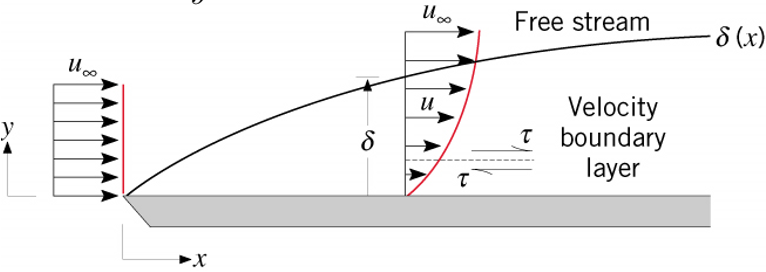
\includegraphics[width = 0.8 \textwidth]{../img/diagram67.png}
  \caption{}
\end{figure}
\subsection{Analysis of order of magnitude}
\begin{align}
  v << u\\
  \left| \frac{\partial}{\partial x} \right| \approx \frac{1}{L}\\
  \left| \frac{\partial}{\partial y} \right| \approx \frac{1}{\delta}
\end{align}
Inside the boundary layer, viscous diffusion is large and of the same order of magnitude of inertial terms, therefore:
\begin{align}
  \frac{u\frac{\partial u}{\partial x}}{\nu\frac{\partial^2 u}{\partial y^2}} \approx 1 \begin{cases}
    u\approx U_\infty\\
    y \approx \delta\\
    x \approx L
  \end{cases} \rightarrow \frac{\frac{U_\infty^2}{L}}{\frac{\nu U_\infty}{\delta^2}} = \frac{\delta^2}{L^2} Re \approx 1
\end{align}
\section{Blasius solution}
In 1908, Blasius found the analytical solution to the flat plate boundary layer problem. The velocity profiles are self-similar at different axial distances from the leading edge.
\begin{gather}
  \eta = \frac{y}{\delta (x)} = \frac{y\sqrt{Re_x}}{x} = \frac{y}{x} \sqrt{\frac{U_\infty x}{\nu}} = y\sqrt{\frac{U_\infty}{x\nu}}\\
  \frac{u}{U_\infty} = f'(\eta)\\
  \frac{v}{U_\infty} = \frac{1}{2} \left( \frac{\nu}{x U_\infty} \right)^{0.5} \left(\eta f'(\eta) - f (\eta)\right)\\
  u \frac{\partial u}{\partial x} + v\frac{\partial u}{\partial y} = \nu \frac{\partial^2 u}{\partial y^2} \rightarrow \frac{1}{2} f(\eta) f''(\eta)+f'''(\eta) = 0
\end{gather}
Boundary conditions:
\begin{gather}
  \begin{cases}
    u = v = 0 & @\  y = 0\\
    u = U_\infty & @\ y = \infty
  \end{cases}\rightarrow \begin{cases}
    f = f' = 0 & @ \ \eta = 0\\
    f' = 1 & @ \ \eta = \infty
  \end{cases}\\
  \frac{\delta}{x} = \frac{A}{\sqrt{Re_x}} \rightarrow A = ?
\end{gather}
Blasius solved this problem and derived the analytical solution, which is shown below:
\begin{figure}[H]
  \centering
  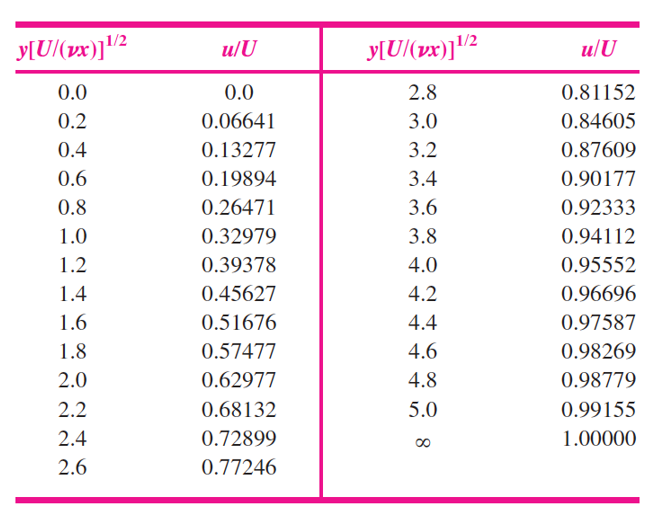
\includegraphics[width = 0.6 \textwidth]{../img/diagram68.png}
  \caption{}
\end{figure}
The boundary layer corresponds to when we have $0.99 U_\infty$, we have $A = 5$, hence:
\begin{align}
  \frac{\delta}{x} = \frac{5}{\sqrt{Re_x}}
\end{align}
Let us look at the shear stress and the friction coefficient:
\begin{align}
  \tau (x) = \mu \left. \frac{\partial u}{\partial y}\right|_{y=0} \rightarrow c_f = \frac{\tau (x)}{\frac{1}{2}\rho U^2_\infty} = \frac{0.664}{\sqrt{Re_x}}
\end{align}
How does the shear stress, $\tau (x)$, vary with distance from the leading edge? If we look at our $Re_x$ term, we see that as $x$ increases $c_f$ decreases. Looking at the gradients of $\frac{\partial u}{\partial y}$ along our boundary layer, we see that the gradient is steeper at $y = 0$. We can also plot $\tau (x)$ against $x$.
\begin{figure}[H]
  \centering
  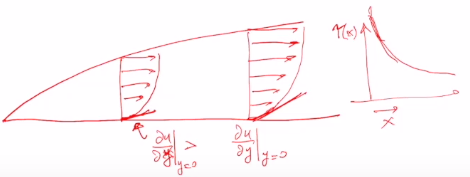
\includegraphics[width = 0.8 \textwidth]{../img/diagram69.png}
  \caption{}
\end{figure}
Let us look at the friction drag on the flat plate:
\begin{figure}[H]
  \centering
  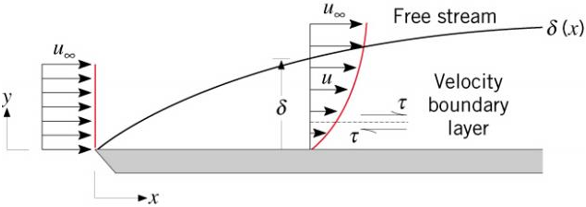
\includegraphics[width = 0.8 \textwidth]{../img/diagram70.png}
  \caption{}
\end{figure}
What is the friction drag on the flat plate per unit of span?
\begin{align}
  D = \int_{0}^{L} \tau(x) \,\mathrm{d}x = 0.664 \rho U_\infty^2 \frac{L}{\sqrt{Re_L}}\\
  c_D = \frac{D}{\frac{1}{2}\rho U_\infty^2 L} = \frac{1.328}{\sqrt{Re_L}} = 2 c_f (L)
\end{align}
\section{Laminar and turbulent profiles}
\begin{figure}[H]
  \centering
  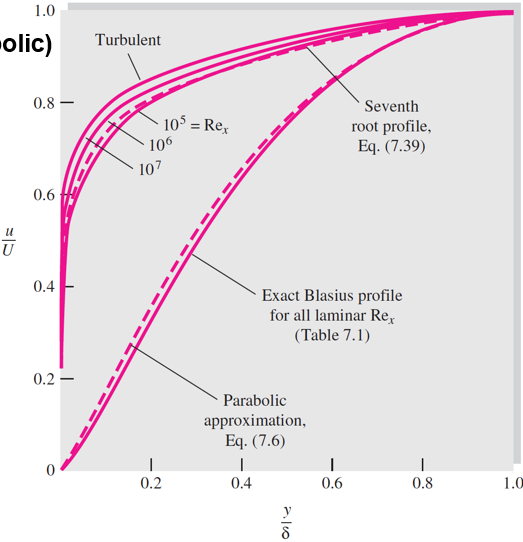
\includegraphics[width = 0.8 \textwidth]{../img/diagram71.png}
  \caption{}
  \label{lamturbpfs}
\end{figure}
Our parabolic approximation is given by the Karman approximation:
\begin{align}
  \frac{u}{U_\infty} = \left( 2 \frac{y}{\delta} - \frac{y^2}{\delta^2}\right)
\end{align}
Turbulent flow can be described as:
\begin{align}
  \frac{u}{U_\infty} = \left(\frac{y}{\delta}\right)^{\frac{1}{5}}
\end{align}
The Prandtl approximation is given as:
\begin{align}
  \frac{u}{U_\infty} = \left(\frac{y}{\delta}\right)^{\frac{1}{7}}
\end{align}
In Figure (\ref{lamturbpfs}), we see that with increasing $Re$, the bulge in our curve also increases. This also means that $\frac{\partial u}{\partial y}$ is also increasing, meaning our shear stress also increases with $Re$.
\subsection{Turbulent friction and drag coefficients}
For $n = \frac{1}{5}$ (fully turbulent flow):
\begin{align}
  \frac{\delta}{x} &= \frac{0.385}{(Re_x)^{\frac{1}{5}}}\\
  c_f &= \frac{\tau (x)}{\frac{1}{2}\rho U_\infty^2} = \frac{0.0594}{(Re_x)^\frac{1}{5}}\\
  c_D &= \frac{D}{\frac{1}{2} \rho U_\infty^2 L} = \frac{0.074}{(Re_L)^{\frac{1}{5}}} = \frac{5}{4} c_f (L)
\end{align}
For $n = \frac{1}{7}$ (fully turbulent flow):
\begin{align}
  \frac{\delta}{x} &= \frac{0.16}{(Re_x)^{\frac{1}{7}}}\\
  c_f &= \frac{\tau (x)}{\frac{1}{2} \rho U_\infty^2} = \frac{0.027}{(Re_x)^{\frac{1}{7}}}\\
  c_D &= \frac{D}{\frac{1}{2}\rho U_\infty^2 L} = \frac{0.031}{(Re_L)^{\frac{1}{7}}} = \frac{7}{6} c_f (L)
\end{align}
\section{Displacement thickness}
\begin{figure}[H]
  \centering
  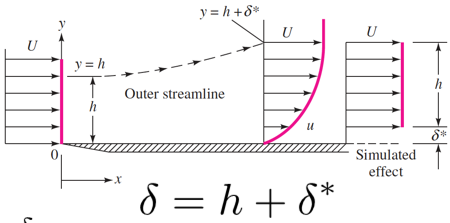
\includegraphics[width = 0.8 \textwidth]{../img/diagram72.png}
  \caption{}
\end{figure}
Based on the conservation of mass; the outer streamline must displace outwards to conserve the mass flow rate. The displacement thickness measure the streamline displacement for different $x$:
\begin{gather}
  \rho U h = \int_{0}^{\delta} \rho u \,\mathrm{d}y = \int_{0}^{\delta} \rho \left(u + U - U\right) \,\mathrm{d}y\\
  Uh = U(h + \delta^*) + \int_{0}^{\delta} \left(u - U\right) \,\mathrm{d}y\\
  \delta^* = \int_{0}^{\delta} \left(1 - \frac{u}{U}\right) \,\mathrm{d}y
\end{gather}
\section{Momentum thickness}
\begin{figure}[H]
  \centering
  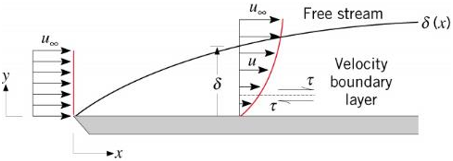
\includegraphics[width = 0.8 \textwidth]{../img/diagram73.png}
  \caption{}
\end{figure}
Based on momentum loss; the total loss os momentum is equivalent to the loss of momentum occurring over a distance $\theta$, denoted as the "momentum thickness."
\begin{gather}
  \rho U^2 \theta = \int_{0}^{\delta} \rho u (U - u) \,\mathrm{d}y\\
  \theta = \int_{0}^{\delta} \frac{u}{U} \left(1 - \frac{u}{U}\right) \,\mathrm{d}y
\end{gather}
\begin{itemize}
  \item The "momentum thickness" measures the deficit in the rate of transport momentum in the layer compared with the rate of transport of momentum in the absence of the layer.
  \item Alternatively it can be seen as the thickness of a completely stagnant layer of fluid giving the same deficit in momentum as the actual profile.
\end{itemize}
For a flat plate (zero pressure gradient), the momentum loss is also equal to the friction drag along the flat plate. 
\begin{gather}
  D = \int_{0}^{\delta} \rho u (U_\infty - u) \,\mathrm{d}y\\
  D = \int_{0}^{x} \tau_w \,\mathrm{d}x\\
  \tau_w = \frac{dD}{dx} = \rho U_\infty^2 \frac{d\theta}{dx}\\
  \frac{\tau_w}{\rho U_\infty^2} = \frac{d\theta}{dx}
\end{gather}
The following equations are valid:
\begin{align}
  c_f = \frac{\tau_w}{\frac{1}{2}\rho U_\infty^2} = 2\frac{d\theta}{dx}
\end{align}
If we know the momentum thickness, I can find the shear stress/friction coefficient on the plate and vice versa.
\section{General case with pressure gradient \& shape factor}
The shape factor is the ratio between the displacement thickness and the momentum thickness.
\begin{align}
  H = \frac{\delta^*}{\theta} = \frac{\int_{0}^{\delta} \left(1 - \frac{u}{U}\right) \,\mathrm{d}y}{\int_{0}^{\delta} \frac{u}{U} \left(1 - \frac{u}{U}\right) \,\mathrm{d}y} > 1
\end{align}
This leads to:
\begin{align}
  \frac{\tau_w}{\rho U_\infty^2} = \frac{d\theta}{dx} + U \frac{dU}{dx} (H + 2)\theta
\end{align}
where $U \frac{dU}{dx} (H + 2)\theta$ is an extra term added due to the presence of a pressure gradient. 
\begin{figure}[H]
  \centering
  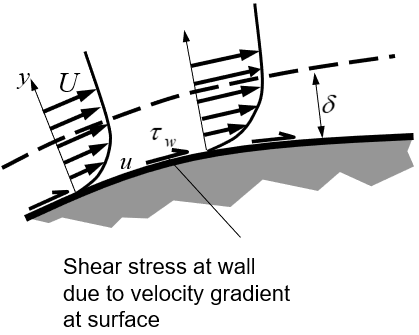
\includegraphics[width = 0.5 \textwidth]{../img/diagram74.png}
  \caption{}
\end{figure}
For laminar flow (flat plate)
\begin{align}
  H = 2.59
\end{align}
For turbulent flow (flat plate)
\begin{align}
  H = 1.29
\end{align}
A large shape factor is indicative of boundary layer separation.
\begin{figure}[H]
  \centering
  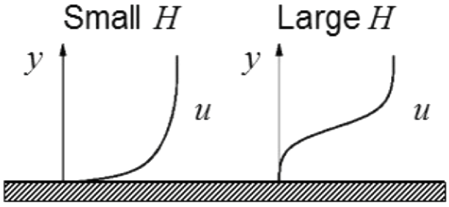
\includegraphics[width = 0.5 \textwidth]{../img/diagram75.png}
  \caption{}
\end{figure}
\section{Laminar - turbulent flow transition}
\begin{figure}[H]
  \centering
  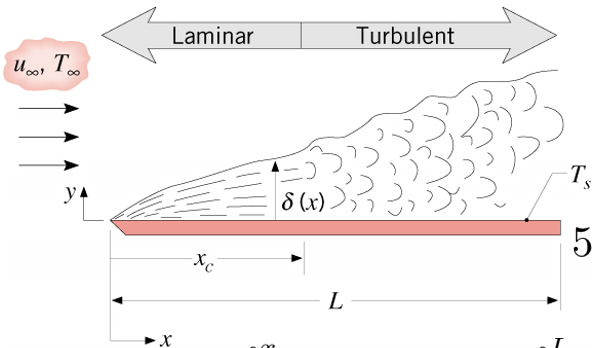
\includegraphics[width = 0.8 \textwidth]{../img/diagram76.png}
  \caption{}
\end{figure}
$x_c$ is defined as the point along our plate where our flow turns turbulent.
\begin{gather}
  Re = \frac{U_\infty x_c}{\nu}\\
\end{gather}
This is normally in the region where $Re = 5 \times 10^5 - 8\times 10^7$.
\begin{align}
  D = \int_{0}^{x_c} \tau_{\textrm{lam}} (x) \,\mathrm{d}x + \int_{x_c}^{L} \tau_{\textrm{turb}} (x) \,\mathrm{d}x\\
  c_D = \frac{1}{L} \left( \int_{0}^{x_c} c_{fl} (x) \,\mathrm{d}x + \int_{x_c}^{L} c_{ft} (x) \,\mathrm{d}x  \right)  
\end{align}
\section{Flat plate drag coefficient}
\begin{figure}[H]
  \centering
  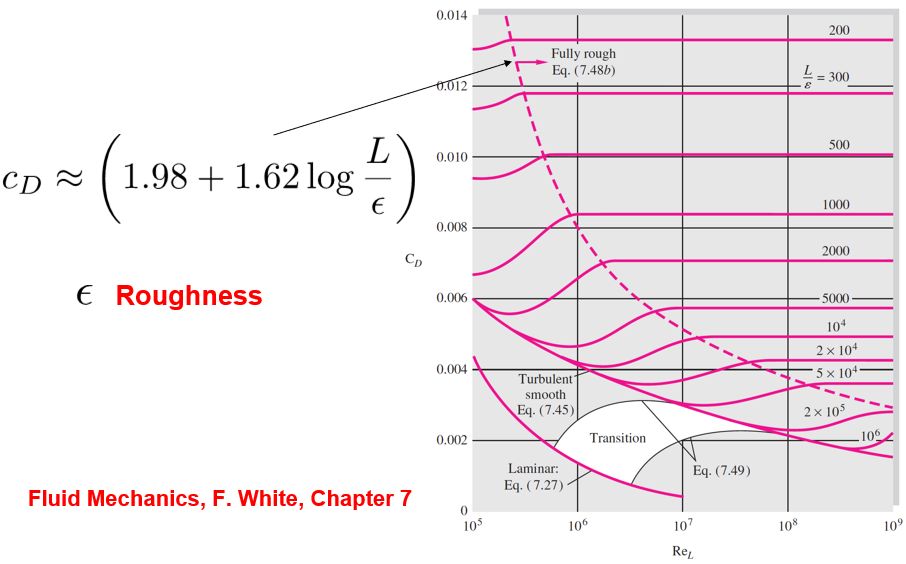
\includegraphics[width = 0.8 \textwidth]{../img/diagram77.png}
  \caption{}
\end{figure}
\end{document}